\documentclass[preview]{standalone}

\title{\vspace{-3em}Semi-Leptonic $t\bar{t}$}
\author{Michael Cardiff}
\date{\today}

%% science symbols
\usepackage{amsmath}
\usepackage{amssymb}
\usepackage{amsthm}
\usepackage{bm}
\usepackage{cancel}
\usepackage{physics}
\usepackage{siunitx}
\usepackage{slashed}

%% general pretty stuff
\usepackage{caption}
\usepackage{float}
\usepackage{graphicx}
\usepackage{url}
\usepackage{enumitem}
\usepackage{hyperref}
\usepackage{tikz}
\usepackage{tikz-feynhand}

% setup options
\captionsetup{labelfont=bf}
\graphicspath{ {./figs/} }

% macros
\renewcommand{\L}{\mathcal{L}}
\renewcommand{\H}{\mathcal{H}}
\renewcommand{\l}{\ell}
\newcommand{\M}{\mathcal{M}}
\newcommand{\mcV}{\mathcal{V}}
\newcommand{\D}{\partial}
\newcommand{\veps}{\varepsilon}
\newcommand{\circled}[1]{\tikz[baseline = (char.base)]{
    \node[shape=circle,draw,inner sep=2pt] (char){#1};}}

% mdframed environments
\usepackage[framemethod=TikZ]{mdframed}
\mdfsetup{skipabove=\topskip,skipbelow=\topskip}
\mdfdefinestyle{defstyle}{%
  linewidth=1pt,
  frametitlerule=true,
  frametitlebackgroundcolor=gray!40,
  backgroundcolor=gray!20,
  innertopmargin=\topskip}

\mdtheorem[style=defstyle]{definition}{Definition}
\mdtheorem[style=defstyle]{theorem}{Theorem}
\mdtheorem[style=defstyle]{problem}{Problem}

\newenvironment{thebook}
{\begin{mdframed}[style=defstyle,frametitle={From the Book}]}{\end{mdframed}}

\begin{document}
% \maketitle

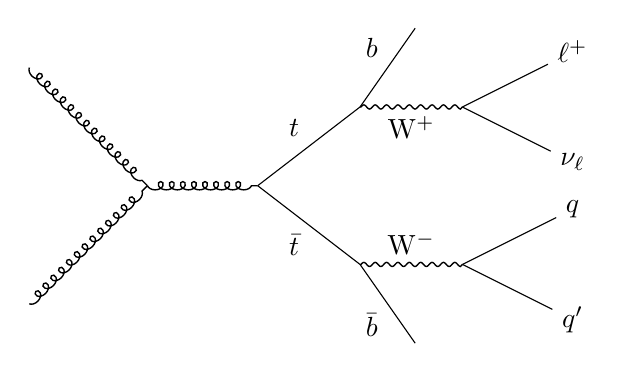
\begin{tikzpicture}
  \begin{feynhand}
    % vertices
    \vertex (g1) at (-1.2,1.5);
    \vertex (g2) at (-1.2,-1.5);
    \vertex (tp) at (3,1);
    \vertex (tb) at (3,-1);
    \vertex (bp) at (3.7, 2);
    \vertex (bb) at (3.7, -2);
    \vertex (wp) at (4.3, 1);
    \vertex (wm) at (4.3, -1);
    \vertex (le) at (5.7,1.7) {$\ell^{+}$};
    \vertex (nu) at (5.7,0.3) {$\nu_\ell$};
    \vertex (q1) at (5.7,-0.3) {$q$};
    \vertex (q2) at (5.7,-1.7) {$q'$};
    \vertex (a) at (0.3,0);
    \vertex (b) at (1.7,0);
    % external particles
    \propag [glu] (g1) to (a);
    \propag [glu] (g2) to (a);
    \propag (wp) to (le);
    \propag (wp) to (nu);
    \propag (wm) to (q1);
    \propag (wm) to (q2);
    \propag (tp) to [edge label=\(b\)] (bp);
    \propag (tb) to [edge label'=\(\bar{b}\)] (bb);
    % internal particles
    \propag [glu] (a) to (b);
    \propag (b) to [edge label=\(t\)] (tp);
    \propag (b) to [edge label'=\(\bar{t}\)] (tb);
    \propag [bos] (tp) to [edge label'=\(\mathrm{W}^{+}\)] (wp);
    \propag [bos] (tb) to [edge label=\(\mathrm{W}^{-}\)] (wm);
  \end{feynhand}
\end{tikzpicture}
\end{document}